\documentclass[12pt, twoside]{article}
\usepackage[letterpaper, margin=1in, head=30pt, headsep=0.1in]{geometry}
\usepackage[english]{babel}
\usepackage[utf8]{inputenc}
\usepackage{amsmath}
\usepackage{amsfonts}
\usepackage{amssymb}
\usepackage{tikz}
%\usetikzlibrary{quotes, angles}

\usepackage{graphicx}
\usepackage{enumitem}
\usepackage{multicol}

\newif\ifmeta
\metatrue %print standards and topics tags

\title{Regents Geometry}
\author{Chris Huson}
\date{October 2021}

\usepackage{fancyhdr}
\pagestyle{fancy}
\fancyhf{}
\renewcommand{\headrulewidth}{0pt} % disable the underline of the header
\raggedbottom


\fancyhead[LE]{\thepage}
\fancyhead[RO]{\thepage \\ Name: \hspace{4cm} \,\\}
\fancyhead[LO]{BECA / Dr. Huson / Geometry 04 Analytic Geometry}

\begin{document}

\subsubsection*{4.6 Slopes of parallel lines}
The slope of a line: $\displaystyle m=\frac{y_2-y_1}{x_2-x_1}$
\begin{enumerate}
\item Do Now: Given $\overleftrightarrow{PQ}$, $P(1,6)$, $Q(3,2)$. Find its slope, $y$-intercept, and equation.
\begin{flushright}
  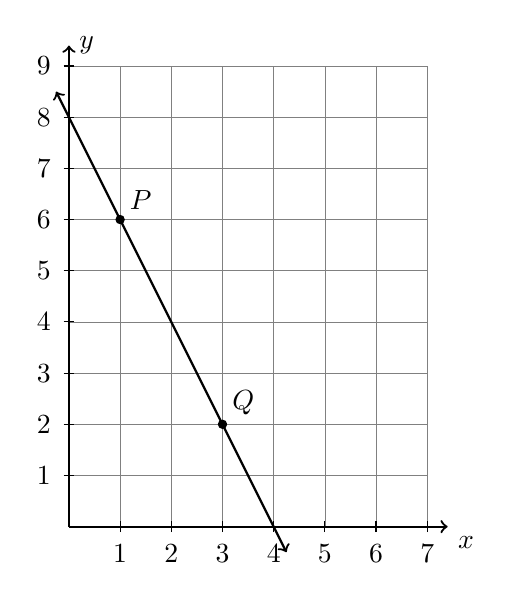
\begin{tikzpicture}[scale=.65]
    \draw [help lines] (0,0) grid (7,9);
    \draw [thick, ->] (0,0) -- (7.4,0) node [below right] {$x$};
    \draw [thick, ->] (0,0)--(0,9.4) node [right] {$y$};
    \foreach \x in {1,...,7}
    \draw[shift={(\x,0)}] (0pt,-3pt)--(0pt,3pt) node[below=5pt] {$\x$};
    \foreach \y in {1,...,9}
    \draw[shift={(0,\y)}] (-3pt,0pt)--(3pt,0pt) node[left=5pt] {$\y$};
    \draw [thick, <->] (-0.25,8.5)--(4.25,-0.5);
    \draw [fill] (1,6) circle [radius=0.08] node[above right] {$P$};
    \draw [fill] (3,2) circle [radius=0.08] node[above right] {$Q$};
  \end{tikzpicture}
  \end{flushright}

\subsubsection*{Parallel lines have the same slope}

\item The line $l$ is shown on the grid below.
\begin{multicols}{2}
\begin{enumerate}
  \item Write down it's slope, $y$-intercept.\\ $m=$
  \hspace{2cm} $b=$
  \vspace{0.25cm}
  \item Write down the equation of line $l$.
  \vspace{1cm}
  \item Draw a line parallel to line $l$ though point $S$.
  \item Write down the equation of the second line.
\end{enumerate}
  \begin{center}
  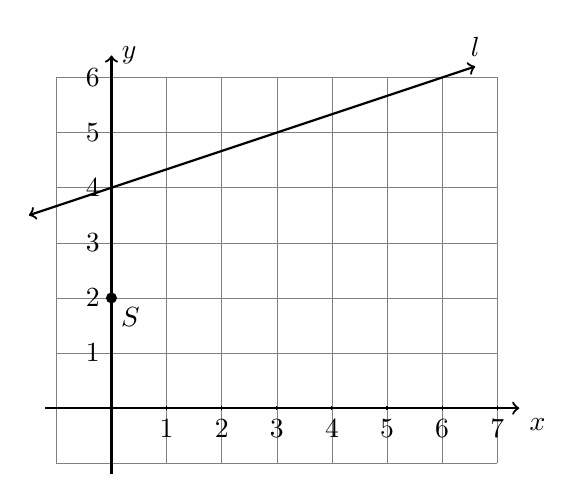
\begin{tikzpicture}[scale=0.7]
    \draw [help lines] (-1,-1) grid (7,6);
    \draw [thick, ->] (-1.2,0) -- (7.4,0) node [below right] {$x$};
    \draw [thick, ->] (0,-1.2)--(0,6.4) node [right] {$y$};
    \foreach \x in {1, ..., 7} \draw (\x cm,1pt) -- (\x cm,-1pt) node[anchor=north] {$\x$};
    \foreach \y in {1,...,6} \draw (1pt,\y cm) -- (-1pt,\y cm) node[anchor=east] {$\y$};
    \draw [thick, <->] (-1.5,3.5) -- (6.6,6.2) node[above]{$l$};
    \fill (0,2) circle[radius=0.1] node[below right]{$S$};
  \end{tikzpicture}
  \end{center}
\end{multicols}\vspace{0.5cm}

\item The line has the equation $y=-x+7$. 
\begin{enumerate}
  \item Write down it's slope and $y$-intercept. \hspace{2cm} $m=$
  \hspace{2cm} $b=$
  \item Is the point $(4, 4)$ on the line? Justify your answer.
\end{enumerate}
\vspace{2cm}

\newpage
\item Graph and label $\triangle CAT$. Calculate the lengths of its sides. $C(2,1)$, $A(12,6)$, $T(12,1)$.
\begin{flushleft}
  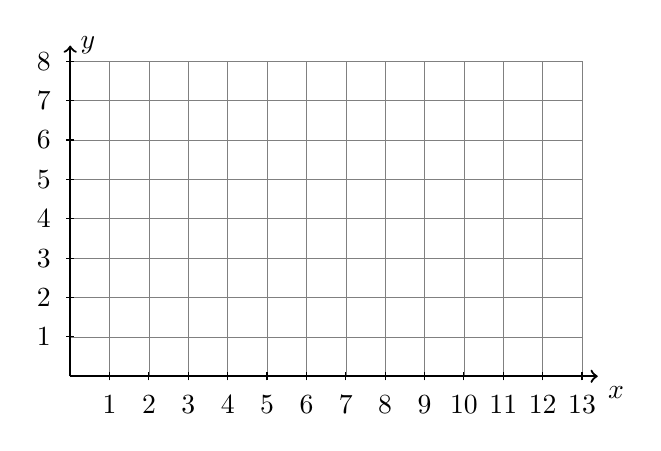
\begin{tikzpicture}[scale=.5]
    \draw [help lines] (0,0) grid (13,8);
    \draw [thick, ->] (0,0) -- (13.4,0) node [below right] {$x$};
    \draw [thick, ->] (0,0)--(0,8.4) node [right] {$y$};
    \foreach \x in {1,...,13}
    \draw[shift={(\x,0)}] (0pt,-3pt)--(0pt,3pt) node[below=5pt] {$\x$};
    \foreach \y in {1,...,8}
    \draw[shift={(0,\y)}] (-3pt,0pt)--(3pt,0pt) node[left=5pt] {$\y$};
  \end{tikzpicture}
\end{flushleft}

\item The base of a right triangle is 4 centimeters long and its hypotenuse is 5 cm. Find its height, $x$ cm.
\begin{flushright}
  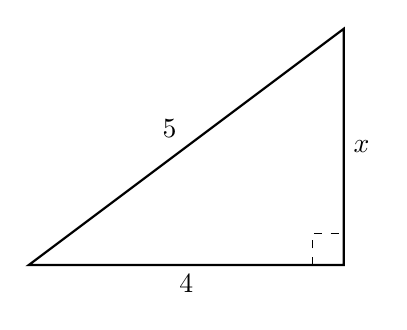
\begin{tikzpicture}[scale=1]
    \node at (2,1.5)[above left]{5};
    \node at (4,1.5)[right]{$x$};
    \node at (2,0)[below]{4};
    \draw [thick] (0, 0)--(4, 0)--(4, 3)--cycle;
    \draw [dashed] (4,0)++(-0.4,0)-- ++(0,0.4)-- +(0.4,0);
  \end{tikzpicture}
\end{flushright}

\item Point $P$ partitions $\overline{MN}$, $M=-6$ and $N=4$, in the ratio $1:4$. Find the value of point $P$. Mark and label $P$ on the graph. \\[1cm]
  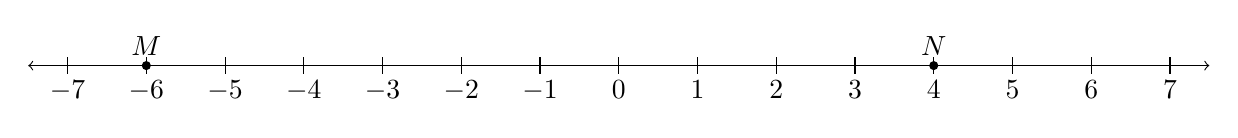
\begin{tikzpicture}
    \draw [<->] (-7.5,0)--(7.5,0);
    \foreach \x in {-7,...,7} %2 leading for diff!=1
      \draw[shift={(\x,0)},color=black] (0pt,-3pt) -- (0pt,3pt) node[below=5pt]  {$\x$};
      \draw [fill] (-6,0) circle [radius=0.05] node[above] {$M$};
      \draw [fill] (4,0) circle [radius=0.05] node[above] {$N$};
  \end{tikzpicture} \vspace{2cm}

\item Given $M(1)$, the midpoint of $\overline{AB}$. Point $A=-3$, find the value of point $B$. Mark and label $B$ on the graph. \\[1cm]
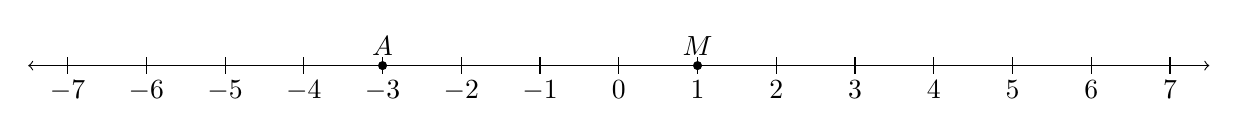
\begin{tikzpicture}
  \draw [<->] (-7.5,0)--(7.5,0);
  \foreach \x in {-7,...,7} %2 leading for diff!=1
    \draw[shift={(\x,0)},color=black] (0pt,-3pt) -- (0pt,3pt) node[below=5pt]  {$\x$};
    \draw [fill] (-3,0) circle [radius=0.05] node[above] {$A$};
    \draw [fill] (1,0) circle [radius=0.05] node[above] {$M$};
\end{tikzpicture}

\end{enumerate}
\end{document}



